\documentclass[11pt, a4paper]{article}

% --- Essential Packages ---
\usepackage[utf8]{inputenc}    % Text encoding
\usepackage{graphicx}          % Required for inserting images
\usepackage{url}               % Required for robust URL handling
\usepackage{hyperref}          % Required for links and URLs
\usepackage{geometry}          % Adjust page margins
\geometry{margin=2.5cm}

% --- Document Information ---
\title{\textbf{Labwork 3 Report: Hello, CUDA!}}
\author{Lucien Elyas Bedrane \\ Student ID: 2640012}
\date{\today}

\begin{document}

\maketitle

% --- Section 1: Objective Breakdown ---
\section{Objectives \& Breakdown}
In this lab, we want to implement a CPU and GPU version of a grayscale function in Python.
This lab was done with Google Collab using the T4 GPU.

% --- Section 2: Code Output Image ---
\section{Implementations \& Results}
For this lab, I mainly used the implementations of grayscale used in the course as well as for the functions to copy data from the CPU to the GPU and to the GPU to the CPU. 
\\From the hints given in the instructions of this labwork, I used the given matplotlib and numpy functions to recover the source image into a 3D array that was then flattened to a 1D array to be used by the grayscale functions later.
\\To test the effect of block sizes and grid sizes on how parallelization allows to increase the GPU calculations, I created a loop that times how long a grayscale iteration takes depending on the block sizes.
\\The following is the graph of Block size vs Time with block size ranging from $2^{0}$ to $2^{10}$:
 
\begin{figure}[h!]
    \centering
    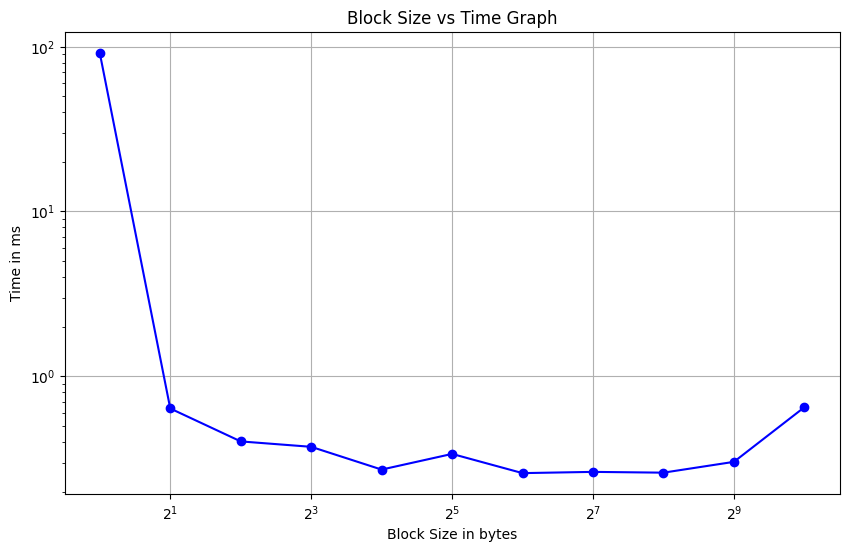
\includegraphics[width=0.8\textwidth]{plots/BlockSize_vs_Time_Graph} 
    \caption{Block size vs Time graph.}
    \label{fig:graph}
\end{figure}

As we can see in this graph, when the block size is $2^{0}$, the time is really bad as it is $10^{2}$ slower than with bigger block size. 
\\We can understand from this that the lower the block size is, the less we can make use of the GPU capacity for parallelization to accelerate its calculations. 
\\However, at a block size of $2^{10}$, a warning is thrown in the execution of our program indicating that we aren't using that many blocks. In other words, we don't utilize the full capacity of the GPU making it that our execution times is slower.
\\Lastly, when the block size is higher than $2^{10}$, the program crashes.

% --- Section 3: Sources ---
\section{Sources \& References}
The following resources and documentation were used to complete this work:

\begin{itemize}
    \item Introduction to CUDA by Tran Giang Son for M2 at ICT\\
    \item Numpy documentation for the reshape function: \\
    \url{https://numpy.org/doc/stable/reference/generated/numpy.reshape.html}

    \item Numpy documentation for the flatten function: \\
    \url{https://numpy.org/doc/stable/reference/generated/numpy.ndarray.flatten.html#numpy.ndarray.flatten}

    \item Matplotlib documentation for the imread function: \\
    \url{https://matplotlib.org/stable/api/_as_gen/matplotlib.pyplot.imread.html}

    \item Matplotlib documentation for the imsave function: \\
    \url{https://matplotlib.org/stable/api/_as_gen/matplotlib.pyplot.imsave.html#matplotlib.pyplot.imsave}
\end{itemize}

\end{document}
